\section{Toolkit Overview}

In this section, we first introduce the design decisions and the
overview of the toolkits. Then we present the user interface and the
major functions.

The toolkit is designed and implemented as a web application, since it
is easiest for crowd workers to visit.

The users of our visualization toolkit include {\em annotation
gatherers} and {\em crowd-source workers}. In general, annotation
gatherers (NLP experts and well-trained programmers) use our toolkit
to collect training data from crowd-source workers for their NLP
systems. We believe annotation gatherers know their NLP problems
better than anyone else, so we leave them to implement a html page to
display their problem. The html page would call the APIs to pass data
(\eg\ objects to cluster) to the toolkits. The core component then is
to visualize the problem, as well as allowing workers to interact with
the objects. Our toolkit keeps the task-visualization transparent to
maximize the flexibility of our toolkit. Figure~\ref{fig:workflow}
shows the workflow of our toolkit.

\begin{figure}
\centering
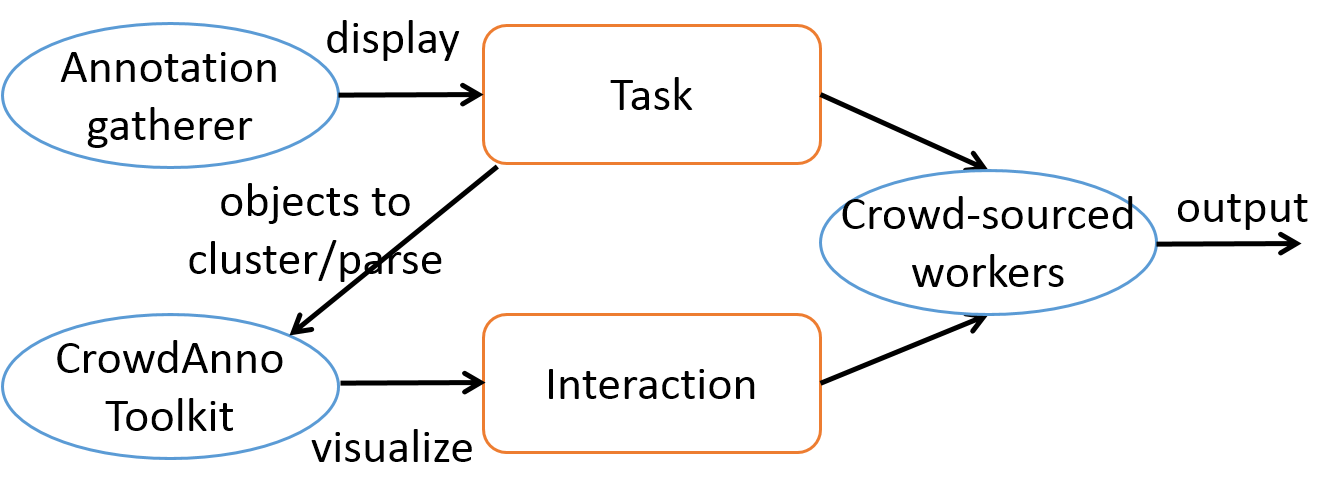
\includegraphics[width=3.1in]{figs/workflow.png}
\caption{Workflow of the toolkit: annotation gatherers generate the
html pages to display the task; our toolkit take the html pages as the
input and visualize the interactions; crowd-sourced workers see the
integrated interface and generate the outputs. }
\label{fig:workflow}
\end{figure}

\subsection{Cluster Labeling}

We use co-reference as the running example for clustering
visualization. Figure~\ref{fig:interface1.png} shows the user
interface. The left sides (about 40\%) displays the NLP task. One simple way to
display the co-reference task, as shown in the figure, is to highlight
the mentions and to give them unique IDs. The right side of the
interface is for the interaction purpose, where workers generate the
clusters interactively. Each token has a corresponding node in the operation area. 
To bridge the connection between the text display and graphic chart, we label each token and its corresponding 
node with the same index. 

\begin{figure*}[th]
\centering
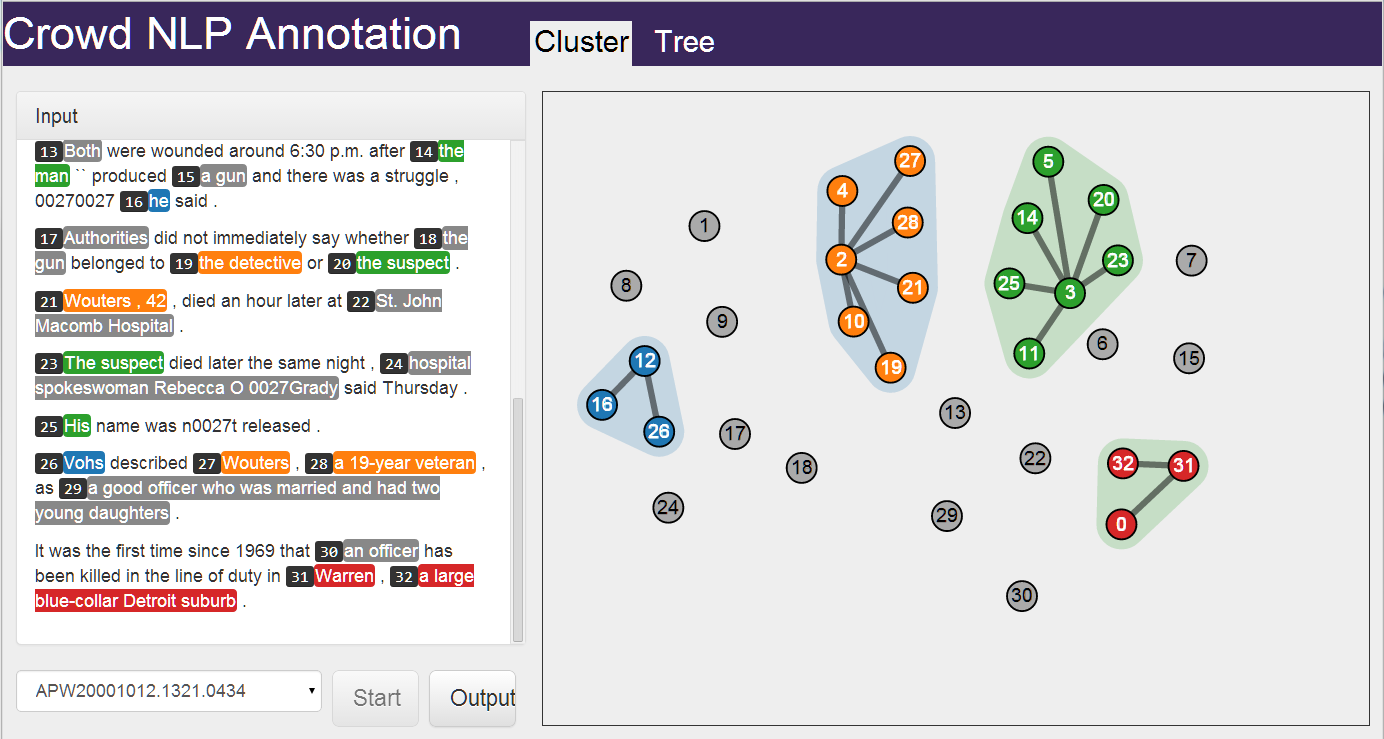
\includegraphics[width=6.1in]{figs/interface1_v2.png}
\caption{Interface of clustering: the left side displays the NLP task, which takes the input from annotator gatherer; the right side is the interaction area, where workers}
\label{fig:interface1.png}
\end{figure*}

Our main manipulation method for clustering two nodes together is dragging nodes and merging into one group. It is the most intuitive operation for one without any instructions to merge two nodes. We will explain the select and drag, link add and remove, and color scheme in the following paragraphs.

\paragraph{\textsc{Select and Drag}\\}
Since we have two separate parts, one for displaying the text, the other for cluster and group manipulation, a proper selection must be supported in order to reduce user's eye movement between two parts. We adopt three mechanism to address this issue. First, if user click on one token, the corresponding node will be highlighted in red color. Similarly when user starts to drag a node, the token is also highlighted in red background. Second, to accelerate tracing from node to the actual text, once user start to drag a node, the display section will scroll to a proper position to let user easily read the context of this token. Third, as shown in Figure \ref{fig:abbrtext}, when drag event starts, an abbreviation text will be displayed under each node so that user can have a brief concept of what each node represents.

\begin{figure}[tH]
\begin{center}
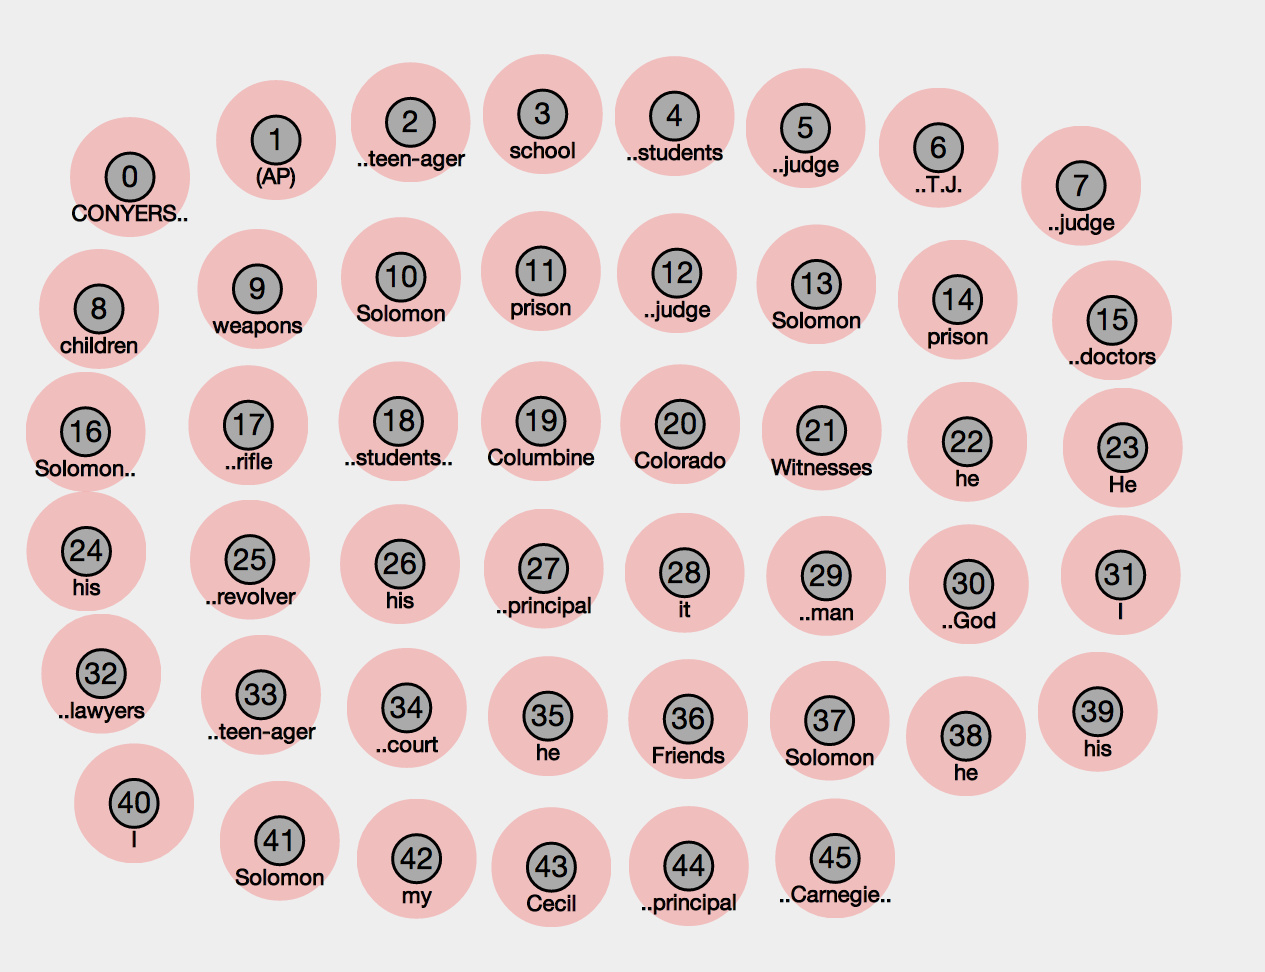
\includegraphics[height=4cm]{figs/abbrText.jpg}
\caption{Abbreviation text is displayed under each node after dragging starts.}
\label{fig:abbrtext}
\end{center}
\end{figure}

\begin{figure}[tH]
\begin{center}
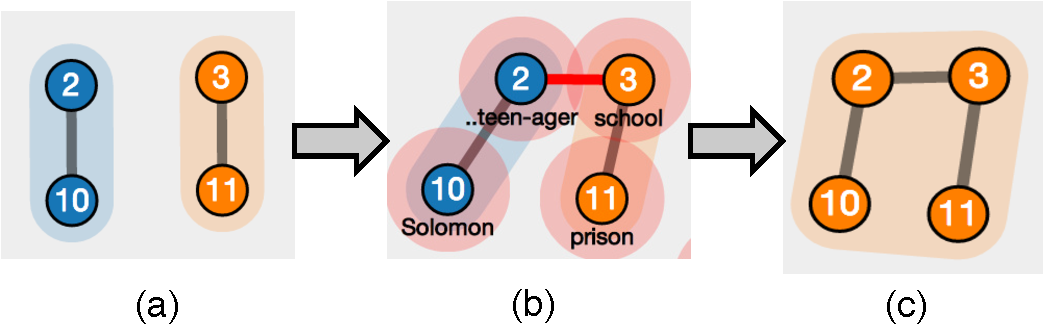
\includegraphics[height=2.5cm]{figs/addlink.pdf}
\caption{(a) before adding the link; (b) in the middle of adding the link; (c) after adding the link.}
\label{fig:addlink}
\end{center}
\end{figure}

\paragraph{\textsc{Link Add and Remove}\\}
Our tool does not allow user explicitly add a link between two nodes. Instead the way to add a link is by dragging a node close enough to the targeted node. Figure~\ref{fig:addlink} shows the process of adding a link. When user starts to drag one node, a shadow circle will be shown around each node. This shadow circle indicates the effective area of adding a link. Once a node is close enough to this shadow circle, a temporary link (in red) will be immediately added to preview the result of this operation (shown in Figure~\ref{fig:addlink}(b)). After user confirms the operation by dropping down the node, a permanent link will be added. Due to the transitivity property of clustering task, \sys\ will automatically bundle two groups together and assign same color for all the nodes in this new group.

The operation that removes a link is as easy as clicking on the link, shown in Figure~\ref{fig:rmlink}. When the mouse hovers over the link, the link color turns to red to indicate that the link will be removed (Figure~\ref{fig:rmlink}(a)). After the click, link will then be removed. If the group is no longer connected after the removement of that link, the system will find out two connected components and separate the original group into two new groups, e.g., Figure~\ref{fig:rmlink}(b).

\begin{figure}[tH]
\begin{center}
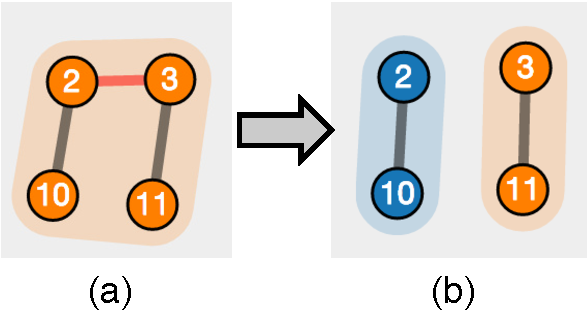
\includegraphics[height=2.5cm]{figs/removelink.pdf}
\caption{(a) in the middle of removing the link; (b) after removing the link.}
\label{fig:rmlink}
\end{center}
\end{figure}

\paragraph{\textsc{Color Scheme}\\}
The token and its corresponding node in the graphic sides have the same color. Any change in the color of the node is also reflected in the corresponding token in the text display part (Figure~\ref{fig:interface1.png}). The consistency in color schemes improves the connection between text and graph part.

The default color is grey. If a node (or token) does not belong to any group, we will use the default color as filling color (or background color). We will assign a new color when a group is generated. If two groups merge together, we will keep the color of group being merged to as the color of new merged larger group (Figure~\ref{fig:addlink}). If a group is splited into two, the majority component keeps the color the origin group. 

\paragraph{\textsc{Group Positioning}\\}
To improve the usability and precision of dragging and adding link operations, and to utilize the space effectively, a proper distance should exist between nodes and nodes, and between groups and groups. We use d3 Force model and calibrate the gravity parameter to enforce a proper gap among the nodes. \sys\ also calculate a proper central point for each group, and impose a force to every nodes inside this group towards that direction. Therefore, groups won't be overlapped in a small region.

\subsection{Tree Construction}

We use syntactic parsing as the running example to show how our
toolkit can build a parsed tree. Figure~\ref{fig:interface_tree.png}
shows the general user interface. The left side is a list of sentences
from which parsing trees are to be built. The right side is the
tree editing area. Three main operations are provided for this task,
i.e. sub-trees grouping by drawing a line over a set of subtrees, node
deletion by drawing a line over the path linking the node to its
parent, and sub-tree collapsing and expansion by clicking on a
sub-tree root. The operations are simple while enough for any tree
building tasks. Figure~\ref{fig:interface2.png} shows how the
trees before and after editing in the interaction area for sentence
{\em ``There is no asbestos in our products now."}. Initially, workers
see a ``flat" tree with sentence tokens as the leaf nodes. They can
merge nodes, insert and delete branch nodes with some intuitive
operators. Note that a valid tree should not change the order of the
leaf nodes. We propose an innovative {\em line-intersect} operator to
guarantee the validity. To our best knowledge, we are the first to
propose this visualization operator on tree structures. We would
introduce them in Section 5.

\begin{figure*}
\centering
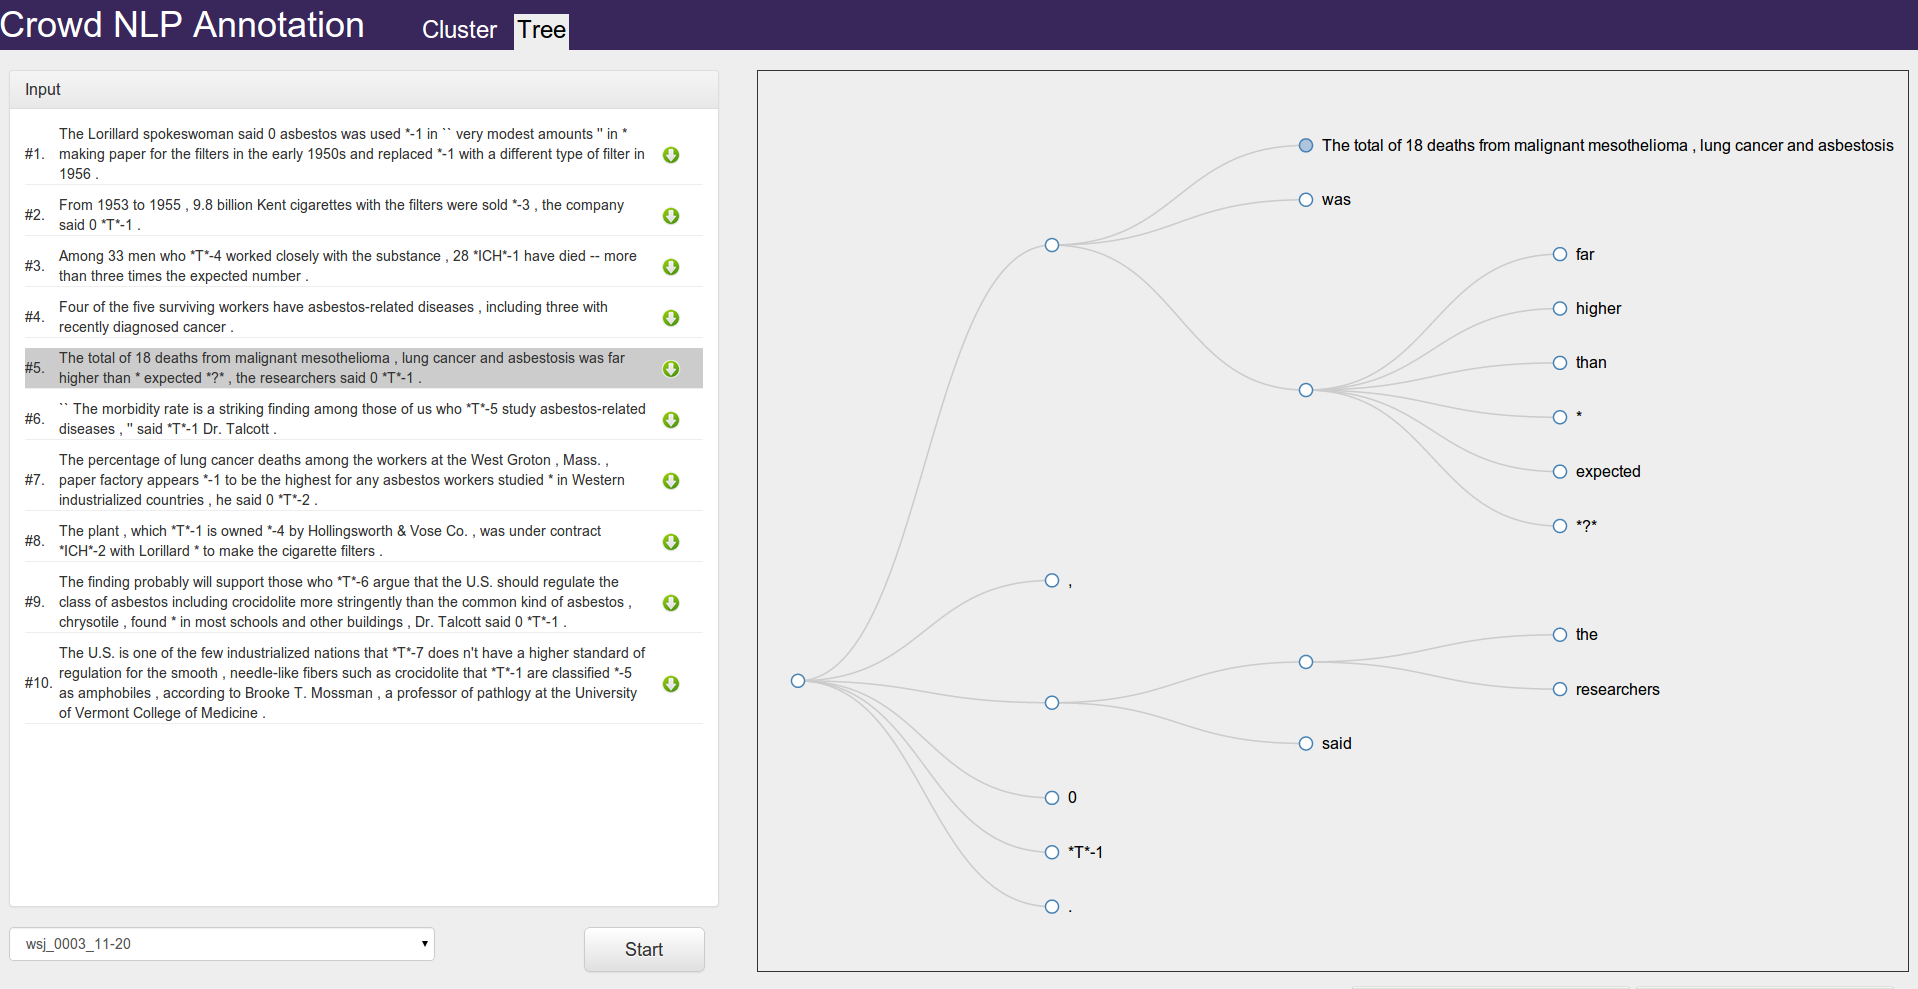
\includegraphics[width=6.1in]{figs/interface-tree.png}
\caption{The before and after trees in the user interface when parsing
the sentence {``There is no asbestos in our products now."}}
\label{fig:interface_tree.png}
\end{figure*}



\begin{figure}
\centering
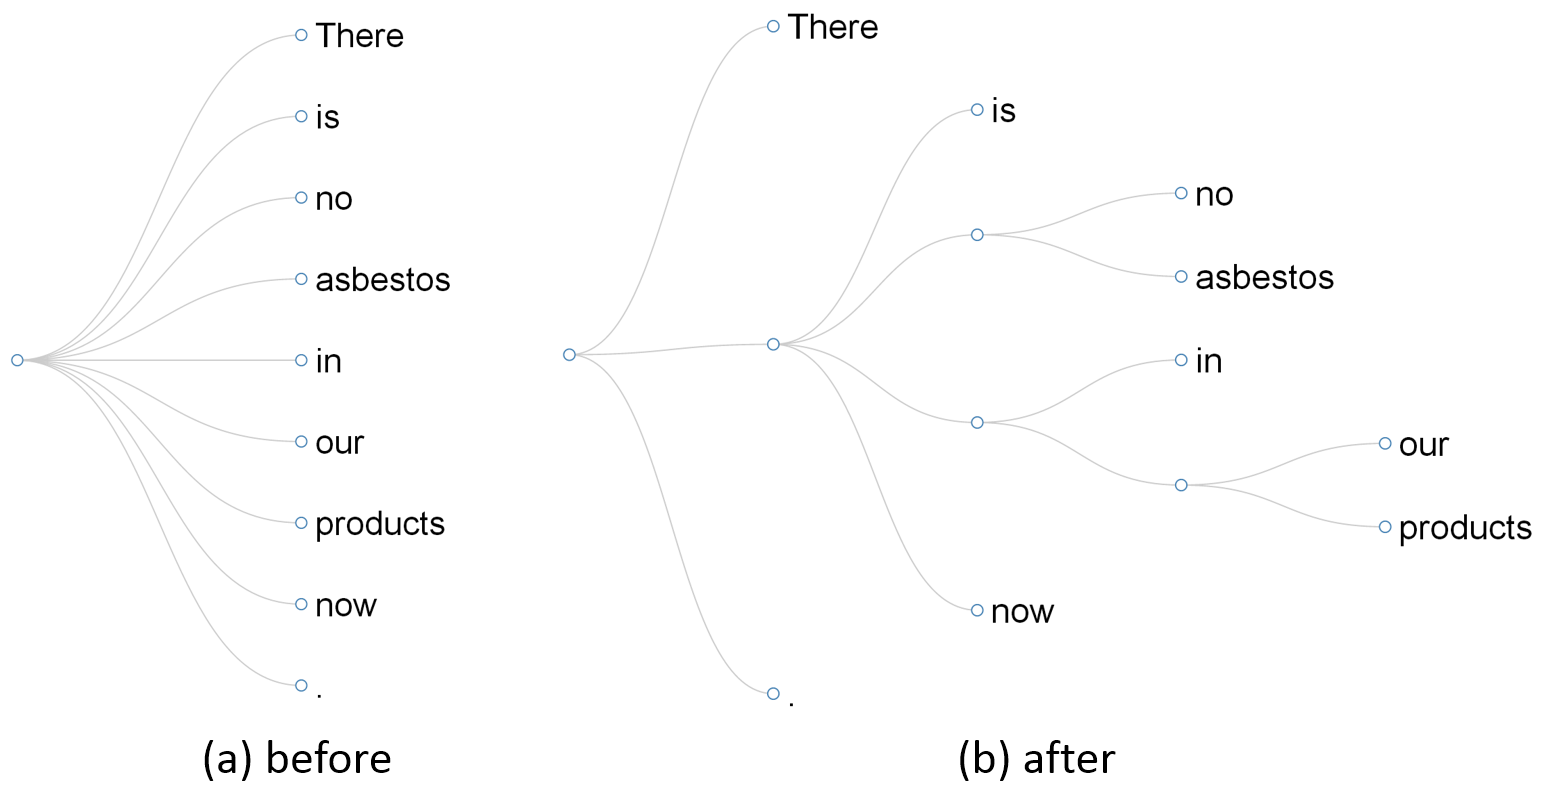
\includegraphics[width=3in]{figs/overview_tree_editing.png}
\caption{The before and after trees in the user interface when parsing
the sentence {``There is no asbestos in our products now."}}
\label{fig:interface2.png}
\end{figure}

